%%%%%%%%%%%%%%%%%%%%%%%%%%%%%%%%%%%%%%%%%
% Journal Article
% LaTeX Template
% Version 1.4 (15/5/16)
%
% This template has been downloaded from:
% http://www.LaTeXTemplates.com
%
% Original author:
% Frits Wenneker (http://www.howtotex.com) with extensive modifications by
% Vel (vel@LaTeXTemplates.com)
%
% License:
% CC BY-NC-SA 3.0 (http://creativecommons.org/licenses/by-nc-sa/3.0/)
%
%%%%%%%%%%%%%%%%%%%%%%%%%%%%%%%%%%%%%%%%%

%----------------------------------------------------------------------------------------
%	PACKAGES AND OTHER DOCUMENT CONFIGURATIONS
%----------------------------------------------------------------------------------------

\documentclass[twoside,twocolumn]{article}

\usepackage[sc]{mathpazo} % Use the Palatino font
\usepackage[T1]{fontenc} % Use 8-bit encoding that has 256 glyphs
\linespread{1.05} % Line spacing - Palatino needs more space between lines
\usepackage{microtype} % Slightly tweak font spacing for aesthetics

\usepackage[english]{babel} % Language hyphenation and typographical rules

\usepackage[hmarginratio=1:1,top=32mm,columnsep=20pt]{geometry} % Document margins
\usepackage[hang, small,labelfont=bf,up,textfont=it,up]{caption} % Custom captions under/above floats in tables or figures
\usepackage{booktabs} % Horizontal rules in tables

\usepackage{lettrine} % The lettrine is the first enlarged letter at the beginning of the text

\usepackage{enumitem} % Customized lists
\setlist[itemize]{noitemsep} % Make itemize lists more compact

\usepackage{abstract} % Allows abstract customization
\renewcommand{\abstractnamefont}{\normalfont\bfseries} % Set the "Abstract" text to bold
\renewcommand{\abstracttextfont}{\normalfont\small\itshape} % Set the abstract itself to small italic text

\usepackage{titlesec} % Allows customization of titles
\renewcommand\thesection{\Roman{section}} % Roman numerals for the sections
\renewcommand\thesubsection{\roman{subsection}} % roman numerals for subsections
\titleformat{\section}[block]{\large\scshape\centering}{\thesection.}{1em}{} % Change the look of the section titles
\titleformat{\subsection}[block]{\large}{\thesubsection.}{1em}{} % Change the look of the section titles

\usepackage{fancyhdr} % Headers and footers
\pagestyle{fancy} % All pages have headers and footers
\fancyhead{} % Blank out the default header
\fancyfoot{} % Blank out the default footer
\fancyhead[C]{} % Custom header text
\fancyfoot[RO,LE]{\thepage} % Custom footer text

\usepackage{titling} % Customizing the title section

\usepackage{hyperref} % For hyperlinks in the PDF
\usepackage{amsmath}
\usepackage[rightcaption]{sidecap}
 
\usepackage{graphicx} %package to manage images
\graphicspath{{images/} }

%----------------------------------------------------------------------------------------
%	TITLE SECTION
%----------------------------------------------------------------------------------------

\setlength{\droptitle}{-4\baselineskip} % Move the title up

\pretitle{\begin{center}\Huge\bfseries} % Article title formatting
\posttitle{\end{center}} % Article title closing formatting
\title{Array lineare di antenna a microstriscia per applicazioni IEEE 802.11} % Article title
\author{%
\textsc{Francesco Morgillo}\\[1ex] % Your name
\normalsize Università degli studi di Genova \\ % Your institution
\normalsize \href{mailto:francesco.morgillo@hotmail.com}{francesco.morgillo@hotmail.com} % Your email address
%\and % Uncomment if 2 authors are required, duplicate these 4 lines if more
%\textsc{Jane Smith}\thanks{Corresponding author} \\[1ex] % Second author's name
%\normalsize University of Utah \\ % Second author's institution
%\normalsize \href{mailto:jane@smith.com}{jane@smith.com} % Second author's email address
}
\date{\today} % Leave empty to omit a date
\renewcommand{\maketitlehookd}{%
\begin{abstract}
\noindent Design of a patch antenna linear array for IEEE 802.11 wireless based application. % Dummy abstract text - replace \blindtext with your abstract text
\end{abstract}
}

%----------------------------------------------------------------------------------------

\begin{document}

% Print the title
\maketitle

%----------------------------------------------------------------------------------------
%	ARTICLE CONTENTS
%----------------------------------------------------------------------------------------

\section{Introduction}


Si vuole progettare un array lineare di 4 antenne a micro-striscia (patch) destinata ad applicazioni wireless con standard IEEE 802.11.
L'antenna dovrà operare nella banda 2400 – 2483.5 MHz che comprende i tipici 12 canali Wi-fi.
In base ai requisiti appena riportati, ricaviamo le seguenti specifiche per l'antenna

\begin{enumerate}[noitemsep] % [noitemsep] removes whitespace between the items for a compact look
\item Frequenza centrale
\item Banda: 
\item Guadagno
\end{enumerate}
 e per l'array
 \begin{enumerate}[noitemsep] % [noitemsep] removes whitespace between the items for a compact look
\item Numero di elementi
\item Tipo schiera
\end{enumerate}

%------------------------------------------------


\section{Singolo elemento}
Il singolo elemento dell'array è costituito da un'antenna a micro-striscia rettangolare.
Viene realizzata su di un substrato di materiale dielettrico, su cui viene fotoinciso uno strato conduttivo di lunghezza L e larghezza W. Sulla faccia opposta del substrato viene posto un piano di massa. L'elemento radiante può essere alimentato in diversi modi: per esempio tramite una linea realizzata in micro-striscia che raggiunge il bordo della patch, oppure con una sonda coassiale che attraversa il substrato.
\subsection*{Geometria}
Il dimensionamento della patch richiede l'impiego di equazioni ricavate con metodi numerici o empirici che tengono conto di effetti fisici dovuti alla complessità e non idealità dell'antenna.
Innanzitutto è necessario tenere presente che per via degli effetti ai bordi, le linee di campo della micro-striscia attraversano due dielettrici differenti, l'aria e il substrato.E' necessario quindi considerare una costante di conducibilità elettrica effettiva $\epsilon_{{reff}}$ che otteniamo è data da 
\begin{equation}
\label{eq:emc}
\epsilon_{reff}= \frac{\epsilon_{r}+1}{2}+\frac{\epsilon_{r}-1}{2}\Big[1+12\frac{h}{W}\Big]^{-\frac{1}{2}}
\end{equation}

Questa quantità corrisponde alla conducibilità elettrica di un materiale dielettrico omogeneo in cui si assume di immergere il modello della microstriscia.

\begin{figure}
  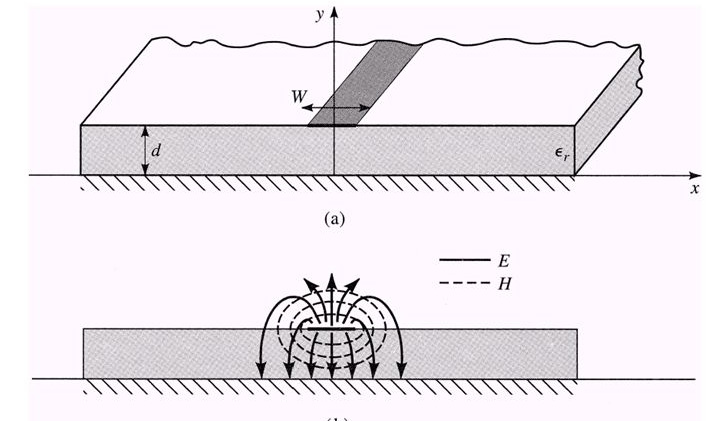
\includegraphics[width=\linewidth]{MICROSTRIPlinefield.jpg}
  \caption{Linee di campo E ed H di una microstriscia.}
  \label{fig:linefield}
\end{figure}
L'effetto ai bordi è poco influente dato che in linea generale \(L/h\gg 1\), ma non può essere ignorato dato che influisce sulla frequenza risonante dell'antenna.


Sempre a causa dell'effetto ai bordi, la lunghezza dell'antenna risulta elettricamente maggiore rispetto alla dimensione reale.
Il campo elettrico che curva attorno le aperture allunga elettricamente ogni lato di una quantità $\Delta L$ .
Un'approssimazione di questa quantità è data da

\begin{equation}
\frac{\Delta L}{h}= 0.412\frac{(\epsilon_{reff}+0.3)\Big(\frac{W}{h}+0.264\Big)}{(\epsilon_{reff}-0.258)\Big(\frac{W}{h}+0.8\Big)}
\end{equation}

Si ha quindi che

\begin{equation}\label{eq:L}
L_{eff}=L+2\Delta L
\end{equation}
dove $L=\lambda/2$ per il modo dominante $TM_{010}$ senza effetto ai bordi.
La frequenza di risonanza è funzione della lunghezza dell'antenna e considerando l'effetto ai bordi è 
\begin{equation} \label{eq:freq}
f_{r(010)}=\frac{1}{2L_{eff}\sqrt{\epsilon_{reff}}\sqrt{\mu_{0}\epsilon_{0}}}
\end{equation}

La larghezza W dell'antenna patch è data da 
\begin{equation}
W=\frac{1}{2f_{r}\sqrt{\mu_{0}\epsilon_{0}}}\sqrt{\frac{2}{\epsilon_{r}+1}}
\end{equation}
mentre combinando la \eqref{eq:freq} e la \eqref{eq:L} si può ricavare la lunghezza L della patch

\begin{equation}
L=\frac{1}{2f_{r}\sqrt{\mu_{0}\epsilon_{0}}\sqrt{\epsilon_{reff}}}-2\Delta L
\end{equation}




Note la frequenza centrale $f_{r}= 2.45GHz$, e considerato il  
substrato di spessore h di 1.6 mm ed $\epsilon_{r}=4.4$,
si ricavano i valori


\begin{center}
\begin{tabular}{ |c|c| } 
 \hline
 W & 35 \\ 
 L & 27.8 \\ 
 $\epsilon_{reff}$ & 4.01 \\
 \hline
\end{tabular}
\end{center}







\subsection{Adattamento di impedenza}

Il metodo più semplice per studiare l'impedenza dell'antenna a micro-striscia è quello di analizzare il suo modello come linea di trasmissione.
L'antenna viene vista quindi come una linea di trasmissione i cui estremi (che corrispondono agli "slot" radianti ai bordi della patch) sono modellati come  due paralleli RC.
I due slot sono identici con ammettenza $Y_{1}=G_{1}+jB_{1}$. Inoltre l'ammettenza totale è puramente reale, data dal parallelo delle due conduttanze  $Y_{in}=Y_{1}+Y_{2}=2G_{1}$ (per via di una "trasformazione di ammettenza"vedi balanis).
Per ricavare il valore di $G_{1}$ si fa riferimento all'equazione 
\begin{equation}
G_{1}= \frac{I_{1}}{120\pi}
\end{equation}
dove 
\begin{align*}
I_{1}= \int_0^\pi \Big[\dfrac{sin (\big( \frac{k_{0}W}{2} cos\theta\big)}{cos\theta}\Big]^2 sin^3\theta d\theta = \\
=-2+cos(X)+XS_{i}(X)+\frac{sinX}{X}
\end{align*}
con 
\begin{equation}
X=k_{0}W
\end{equation}

Nota $G_{1}$ si può dedurre la resistenza in ingresso $R_{in}$ della patch dato che 
\begin{equation}
R_{in}=Z_{in}= \frac{1}{Y_{in}}=\frac{1}{2G_{1}}
\end{equation}

Si modifica questa espressione in modo tale da considerare gli effetti di accoppiamento fra i due slot.

\begin{equation}
R_{in}=Z_{in}= \frac{1}{Y_{in}}=\frac{1}{2G_{1}+2G_{12}}
\end{equation}
Il valore di conduttanza mutua si approssima con 
\begin{equation}
G_{12}=int=Z_{in}= \frac{1}{Y_{in}}=\frac{1}{2G_{1}}
\end{equation}

%------------------------------------------------




%------------------------------------------------




%----------------------------------------------------------------------------------------
%	REFERENCE LIST
%----------------------------------------------------------------------------------------

\begin{thebibliography}{99} % Bibliography - this is intentionally simple in this template

\bibitem[Figueredo and Wolf, 2009]{Figueredo:2009dg}
Figueredo, A.~J. and Wolf, P. S.~A. (2009).
\newblock Assortative pairing and life history strategy - a cross-cultural
  study.
\newblock {\em Human Nature}, 20:317--330.
 
\end{thebibliography}

%----------------------------------------------------------------------------------------

\end{document}
